\documentclass{article}

% Language setting
\usepackage[english]{babel}

% Page size and margins follow the cryptography-research manuscript format.
\usepackage[letterpaper,top=2cm,bottom=2cm,left=3cm,right=3cm,marginparwidth=1.75cm]{geometry}

% Useful packages
\usepackage{amsmath,amsthm,amsfonts,amssymb,tikz,booktabs,arydshln,colortbl,caption,float,placeins}
\usepackage{graphicx,multirow,url,natbib}
\usepackage[colorlinks=true,allcolors=blue]{hyperref}
\usepackage{fancyhdr}
\usepackage{algorithmicx}
\usepackage[ruled]{algorithm}
\usepackage{algpseudocode}
\usetikzlibrary{arrows.meta,positioning}

\fancyhf{}
\renewcommand\headrulewidth{0pt}
\pagestyle{fancy}

\title{Lockstep: Bit-Exact, Verifiable Transformer Inference at Parity Across Devices,\\
for Dense and Mixture-of-Experts Models}
\date{Version 0.2.0, 10 September 2026}
\author{Perica Glavas\\ \small\texttt{pg@lambda.so} \and Maksym Yakovenko\\ \small\texttt{max@lambda.so} \and Logan Allen\\ \small\texttt{logan@nationalcompute.io}}

\newtheorem{Thm}{Theorem}[section]
\newtheorem{Prop}[Thm]{Proposition}
\newtheorem{Lem}[Thm]{Lemma}
\newtheorem{Corr}[Thm]{Corollary}
\newtheorem{Algo}[Thm]{Algorithm}
\newtheorem{Example}[Thm]{Example}
\newtheorem{Prot}[Thm]{Protocol}
\newtheorem{Def}{Definition}[section]
\newtheorem{Fact}{Fact}[section]
\newtheorem{Ass}{Assumption}[section]
\newtheorem{Rem}[Thm]{Remark}


\newcommand{\Fth}{\mathbb{F}_{32}}
\newcommand{\Bf}{\mathbb{B}_{16}}
\newcommand{\fl}{\operatorname{fl}_{32}}
\newcommand{\bfround}{\operatorname{bf}_{16}}
\newcommand{\rne}{\operatorname{RNE}}
\newcommand{\rescale}{\operatorname{rescale}}
\newcommand{\LSSA}{\mathsf{LSSA\mbox{-}B8}}
\newcommand{\Enc}{\operatorname{Enc}}
\newcommand{\Hash}{\operatorname{H}}

\begin{document}

\maketitle

\begin{abstract}
A computation can be verified only relative to a single correctness relation.  Production
Transformer serving does not provide one at the bit level: mathematically equivalent
kernels, reduction orders, batch compositions, compilers and devices legitimately return
different floating-point bit strings, so an auditor must either reproduce the provider's
environment or accept a tolerance.  Recent work shows both escapes are weak: batch-invariant
engines hold only within one GPU family, and a one-bfloat16-spacing tolerance is blind to an
entire class of epilogue faults.

This paper presents \emph{Lockstep}, which makes the served inference function itself
canonical.  A versioned contract replaces implementation-selected floating-point behaviour
with bounded integer arithmetic, immutable lookup tables, and a small ordered set of
explicitly rounded binary32 operations; the same contract is evaluated by an optimized
serving engine and by a portable CPU reference, and correctness is bit equality to a public
function.  Lockstep Softmax Attention (LSSA-B8) uses per-block power-of-two quantization,
exact int32 score and value products, a digest-pinned 8-bit exponential table and a
committed two-level binary32 fold.  A companion contract covers linears, an index-pinned
float RMSNorm, rotary embeddings, SiLU, the language-model head and tensor-parallel
reduction, and a mixture-of-experts contract covers the router, expert dispatch and combine,
including a rule that consumes MXFP4 expert weights exactly without requantization.

The contract is implemented as a vLLM plugin.  Against a clean stock vLLM on the same H100,
Qwen2.5-7B, Llama-3.1-8B, Mistral-7B, Phi-4-mini and Qwen3-8B serve at or above stock on
single-stream decode at every batch and on 2K--8K prompts, within 6\% at 32K; the
mixture-of-experts model Qwen3-30B-A3B serves at 1.32--1.37$\times$ stock throughput under 64
concurrent chat requests, and GPT-OSS-20B runs exactly on its native MXFP4 weights at
0.52--0.54$\times$.  Every
kernel is gated bit-identical to the reference, the engine's perplexity readings are
identical across runs, the same source yields identical digests on Hopper, Ada and
Blackwell GPUs, and the norm reference is reproduced bit for bit on x86 and ARM CPUs.  A Lean~4 development mechanizes the contract core: executable bit-level binary32 and
bfloat16 semantics, the integer bounds, the ordered fold's determinism and its legal
schedule refinements, and sound admission, trace and audit checkers, bridged to an
independent Python verifier; CUDA correspondence stays gate-based.  We state precisely what
these mechanisms establish, show why an exact-MXFP4 rule has a structural speed floor while the int8 expert rule serves
above stock, and set out the remaining step to full semantics: an executable interpreter that is
itself the specification, bound to a signed commitment.
\end{abstract}

\section{Introduction}
\label{sec:introduction}

A public model checkpoint is not yet a public computation.  It specifies tensors and a
high-level graph, but a production engine still chooses kernels, floating-point reduction
trees, fusion boundaries, cache layouts, batching schedules and collective orders.  Those
choices are normally treated as implementation detail because their outputs are numerically
close.  For verification they are semantic: if several output bit strings are all
``correct,'' there is no unique statement for a verifier to check.

Two responses have emerged in the past year.  The first fixes the engine: batch-invariant
kernels with fixed reduction trees make one engine reproduce itself run after run
\cite{he2025nondeterminism,sglang2025deterministic,eigenai2026,llm42}.  Their authors are
explicit that the property holds within one GPU family; the ``reference'' is whatever the
chosen kernel computes.  The second fixes the verifier: emulate a declared GPU's tensor-core
arithmetic on a CPU so its bits can be reproduced elsewhere \cite{badash2026hawkeye,mmasim2025,
cankaya2026bitexact}.  That reference is architecture-specific and must be rebuilt for every
hardware generation.  A third response, tolerance-based conformance, has been measured and
found wanting: Chen shows that every epilogue fault in an int8 pipeline moves an output by at
most one bfloat16 spacing, so that four of the five are detected by no check of a suite that
accepts one spacing, and the fifth only under power-of-two scales \cite{chen2026pow2}.

The advance in this work is to move the boundary of specification.  Lockstep does not wrap a
proof around an underspecified floating-point server, nor force every implementation of
conventional softmax through one GPU instruction trace.  It defines a new, versioned
inference function whose mathematical structure admits both a production GPU implementation
and a direct portable reference with exactly the same bits, and it chooses that function
jointly with the kernel architecture so that the production path stays at stock speed.

\begin{samepage}
\begin{Def}[Canonical inference contract]
\label{def:canonical-contract}
For contract version $v$, let $\mathcal{D}_v$ be the admitted set of manifest-bound model
constants, tokenized requests, public decoding parameters, and, for randomized sampling, an
explicit random tape.  A \emph{canonical inference contract} is a function
\begin{equation}
  F_v:\mathcal{D}_v\longrightarrow\{0,1\}^{\star}
  \label{eq:canonical-function}
\end{equation}
whose output encodes the model result and its auditable intermediate rows.  Every arithmetic
operation, constant, rounding point, state transition, reduction order and exceptional case
that can change this bit string is fixed by $v$.  Hardware mapping, batch composition and
kernel tiling may vary only where the contract proves or directly specifies them to be
bit-inert.  Inputs outside $\mathcal{D}_v$ must be refused rather than silently routed to a
different function.
\end{Def}
\end{samepage}

A production implementation $P_v$ and reference implementation $R_v$ are compliant when
$P_v(z)=R_v(z)=F_v(z)$ for every $z\in\mathcal{D}_v$.  This separates three questions that
conventional inference conflates: \emph{semantics} (is there exactly one declared output bit
string?), \emph{implementation} (does the optimized engine evaluate that function?), and
\emph{evidence} (what binds a deployment or request to that engine?).  The contract answers
the first; reference equivalence, kernel gates and end-to-end fingerprints address the
second; commitments and replay address the third.

\begin{center}
\fbox{\begin{minipage}{0.90\textwidth}
\textbf{Core idea.}
Turn inference from an implementation-dependent numerical procedure into a canonical
execution relation, while designing that relation so its dominant work remains
accelerator-efficient.  Once the production kernel and a portable reference compute the same
function, verification can use bit equality: there is one accepted result, and an
authenticated differing bit is a concrete witness of nonconformance.
\end{minipage}}
\end{center}

\subsection{Design rationale}

Attention is where long reductions, exponentials, causal scheduling and a persistent KV
cache meet.  Serializing a conventional floating-point implementation would define one
result but discard the tiling and parallelism on which serving depends; demanding arbitrary
schedule invariance from binary32 addition is impossible without a different accumulator.
LSSA-B8 divides the work along an arithmetic boundary: scores and 128-key value partials are
bounded exact integers and may be tiled freely; only a small state crosses blocks, and that
state follows a published order with explicit rounding.  The contract grants freedom where
algebra supports it and removes it where finite-precision arithmetic does not.

The same discipline extends to every other operator, and Section~\ref{sec:moe} shows that it
extends to a mixture of experts: the router's scores are integer table values with a declared
tie rule, dispatch is a permutation, the expert matmuls are int8 with the same epilogue as the
dense linears, and the combine is an ascending-index fold.  For a model shipped with
microscaling MXFP4 experts, the contract can consume the published 4-bit weights exactly,
with a declared per-block rounding sequence, so no requantization stands between the public
checkpoint and the served function.

\subsection{Contributions}

\begin{enumerate}
  \item \textbf{A canonical serving abstraction and its evidence ladder.}
  Definition~\ref{def:canonical-contract} states the object required for exact
  cross-platform inference, separates semantic, implementation and deployment evidence, and
  Section~\ref{sec:nextsteps} defines the last step to full semantics: an executable
  interpreter that is the specification, bound to a signed root.

  \item \textbf{A bit-exact attention construction.}  LSSA-B8 combines per-block
  power-of-two quantization, exact integer score and value partials, a digest-pinned
  exponential table and a committed two-level binary32 fold.  We prove integer safety, legal
  scheduling freedoms, split-KV equivalence and cross-platform bit reproducibility.

  \item \textbf{Complete decoder and mixture-of-experts contracts.}  Version 2.6 fixes
  int8 linears with a declared outlier side path, a float RMSNorm whose reduction order is
  pinned by element index and whose reciprocal square root is one IEEE square root and one
  IEEE division, fixed-Q14 rotary embeddings, table SiLU, a two-plane language-model head,
  basis rotations and a rank-ordered tensor-parallel reduction.  Version 3 adds an int8 gate,
  a table router with a lowest-index tie rule, int8 experts under the dense contract, an
  ascending-index combine, an addendum for GPT-OSS's biased clamped SwiGLU, and a rule that
  consumes MXFP4 expert weights exactly: per 32-wide block an exact int32 partial and one
  rounded binary32 update in ascending block order.

  \item \textbf{A production implementation at parity.}  A vLLM plugin evaluates prompt rows
  inside a modified FlashAttention-3 kernel, generated rows in a pipelined split-KV kernel,
  the dense stack in fused CUDA kernels, and the MoE block in grouped int8 and
  MXFP4-consuming kernels.  Five dense families serve at or above stock on decode at every
  batch and on 2K--8K prompts; Qwen3-30B-A3B serves at 1.32--1.37$\times$ stock.

  \item \textbf{An evidence chain across devices, and a precise account of the floor.}  A
  scalar golden, torch references, standalone gates with negative controls, live row replay,
  a manifest fingerprint, and a cross-architecture kit whose 538 output digests are identical
  on Hopper, Ada and Blackwell, with the float norm's reference reproduced on x86 and ARM
  CPUs; a Lean~4 mechanization of the contract core with an exported artifact checked by an
  independent Python bridge; and an arithmetic account of why the exact-MXFP4 rule sits
  below parity while the int8 expert rule does not.
\end{enumerate}

\subsection{Scope of claims}

The exactness claim is \emph{contract exactness}: equal contract-versioned inputs and
constants imply equal output bits.  LSSA-B8 approximates real-valued softmax; it does not
reproduce softmax's output bits, and approximation quality is measured against the original
bf16 model.  Canonical execution is not a cryptographic proof: a manifest hash binds public
artifacts, a fingerprint shows that a live engine reproduces one prepared probe, and a
post-commitment sampled replay detects incorrect committed rows with the probability derived
in Section~\ref{sec:audit}.  Succinct verification of every row requires composition with a
proof system.  Finally, the served function is canonical for every operator the contract
covers; Section~\ref{sec:nextsteps} names what the contract does not yet cover (the decode
loop's tie and sampling rules, and the attention of one model family) and how it will.

\section{Background and Related Work}
\label{sec:background}

Lockstep lies at the intersection of numerical reproducibility, efficient attention,
quantized inference, executable specification and verifiable computation.  Each line
contributes a necessary idea; none by itself supplies a canonical production LLM server.

\subsection{Numerical reproducibility and batch-invariant engines}

IEEE-754 defines formats and rounding for individual operations
\cite{ieee754,goldberg1991floating}, but the real-number expression $a+b+c$ does not select
between $\fl(\fl(a+b)+c)$ and $\fl(a+\fl(b+c))$.  Reproducible summation research showed
that order-independent reductions can be built by changing the accumulator
\cite{demmel2013reproducible}: reproducibility is an algorithmic property, not a flag.

The 2025--2026 batch-invariance line applied this to serving.  Thinking Machines traced
run-to-run nondeterminism to batch-size-dependent reduction trees and rewrote RMSNorm, GEMM
and attention with fixed strategies, reaching identical outputs across 1,000 runs at about
twice the latency \cite{he2025nondeterminism}; SGLang and vLLM shipped deterministic modes
with lower overhead \cite{sglang2025deterministic,vllm2026batchinvariance}; EigenAI reports
canonical tree reductions at 97--99\% of cuBLAS and states that ``determinism currently holds
only within fixed GPU families,'' with zero matches between A100 and H100 \cite{eigenai2026};
LLM-42 verifies windows of tokens under a canonical replay shape \cite{llm42}.  vLLM's mode covers the fused MoE path since mid-2026 \cite{vllm2026batchinvariance}.
These systems solve a narrower problem than ours: each defines its reference as one kernel's
behaviour on one hardware family, so a CPU or a different GPU cannot evaluate it.
(FlashAttention's own \texttt{deterministic} flag concerns the backward pass; forward
nondeterminism in serving comes from split-KV and batch composition.)  Lockstep places the
arithmetic in a public contract, so a CPU reference and a GPU kernel can be different
programs sharing one result.

\subsection{Hardware-specific arithmetic reproduction}

Hawkeye recovers hidden Tensor Core accumulation semantics---product grouping, internal
precision, truncation, normalization, subnormal handling---and encodes them in an
architecture-specific CPU emulator \cite{badash2026hawkeye}; MMA-Sim characterizes nine
distinct matrix-multiply algorithms across ten architectures \cite{mmasim2025}; Cankaya
re-executes native kernels bit-exactly on a CPU without changing the served model
\cite{cankaya2026bitexact}.  These measurements show why ``matrix multiplication'' is not one
cross-hardware function: Ampere FP16 accumulation uses a two-stage tree with a 24-bit
significand where Hopper combines the accumulator and all products in one stage with 25 bits.

Lockstep chooses the opposite semantic anchor.  Hawkeye asks ``what bits did this declared
GPU produce?'' and makes the verifier emulate that GPU; Lockstep asks ``what bits does the
public contract require?'' and makes the serving implementation evaluate that
architecture-independent function.  Hawkeye preserves an existing GPU arithmetic path and
moves exact reproduction to the auditor; Lockstep changes the served function and bears the
kernel-engineering and approximation cost.  In return, its reference does not emulate a GPU,
and its contract extends through attention, nonlinearities, state transitions, expert routing
and tensor-parallel reduction, which the emulation line leaves to future work.  The approaches
are complementary.

\subsection{Online softmax and tiled attention}

The Transformer made scaled dot-product attention the central sequence operation
\cite{vaswani2017attention}.  Online softmax showed that a running maximum and normalizer can
be updated in one pass \cite{milakov2018online}; FlashAttention turned that recurrence into
an IO-aware tiled algorithm \cite{dao2022flashattention}, FlashAttention-3 mapped it to
Hopper with warp specialization and asynchronous transfers \cite{shah2024flashattention3},
and vLLM made the KV cache pageable \cite{kwon2023pagedattention}.  ``Exact attention'' in
that literature means exact relative to the mathematical formula, not that every legal
finite-precision tile order yields one bit string.  LSSA preserves the block-state
architecture while replacing its semantics: table weights and integer block partials carry
most of the work, and the cross-block recurrence is explicitly ordered.

\subsection{Quantized inference and power-of-two arithmetic}

LLM.int8() routes outliers separately \cite{dettmers2022llmint8}, SmoothQuant moves
activation difficulty into weights \cite{xiao2023smoothquant}, and I-BERT replaces
nonlinearities with integer approximations \cite{kim2021ibert}.  KIVI and KVQuant quantize
the KV cache for memory \cite{kivi2024,kvquant2024}.  The Open Compute microscaling formats
standardize block-scaled 4-bit weights \cite{mxfp4}, which GPT-OSS ships natively
\cite{gptoss2025}.

Integer-only Transformers extend I-BERT's programme to vision and language models with
fully integer softmax and normalization \cite{ivit2023,illm2024}; their goal is an
integer datapath, not a public relation, and their reductions stay implementation-ordered.
Long (Kulisch) accumulators are the classical alternative to a committed fold: an exact
fixed-point sum of all products \cite{kulisch2013}; LSSA uses bounded integer partials
inside a block for the same reason and accepts a short ordered binary32 recurrence across
blocks because the value dynamic range across a 128k-key context does not fit a practical
accumulator.  Two contemporaneous works reach for power-of-two scales for reasons adjacent to
ours.  Chen
requantizes int8 weight scales to their nearest power of two and finds that CUTLASS and
Triton then agree bitwise at every linear layer (196/196 and 252/252, against 8/196 and
10/252 under the checkpoints' own scales), yielding byte-identical generated tokens at 1.7B,
8B and 14B with perplexity changes of $+0.32\%$, $-0.28\%$ and $+0.48\%$
\cite{chen2026pow2}.  That is precisely the trade our int8 expert and linear rules make, and
it is an independent measurement of its quality cost.  Shift-Accumulate Attention quantizes
keys to signed power-of-two codes so the score product needs no multiplier, reporting
$4.6\times$ the attention throughput of FP16 at 32K context on an RTX 4090 for
TinyLlama-1.1B \cite{ahmed2026shiftacc}; its goal is efficiency, its reference matches the
kernel to a tolerance of $2\times10^{-4}$, and it does not address the softmax fold, engine
integration or verification.  Lockstep uses quantization for an additional reason: bounded
integer arithmetic restores associativity inside the ranges the contract proves, so integer
tiles can be rescheduled without changing a partial, and lookup tables turn transcendental
operations into finite public constants.

\subsection{Verifiable inference}

SafetyNets expresses restricted networks as arithmetic circuits with an interactive proof
\cite{ghodsi2017safetynets}; Slalom protects nonlinear work in a trusted execution
environment \cite{tramer2019slalom}; ZKML and zkLLM optimize zero-knowledge circuits for
inference \cite{chen2024zkml,sun2024zkllm}; DeepProve and NanoZK prove GPT-2- to
Llama-2-class models over field integers with quantized weights and tabulated nonlinearities
\cite{deepprove2026,nanozk2026}.  Refereed delegation (Verde) bisects a dispute to one
operator and requires bitwise reproducibility between referee and workers, supplied by
fixed-order float operators at 30--60\% overhead \cite{verde2025}; TAO and VeriLLM relax
this to per-operator tolerances and report residual attack success under worst-case IEEE
bounds \cite{tao2025,verillm2025}.  TEE attestation on H100 measures firmware, driver and
enclave but not weights, kernel selection or numerics \cite{nvidia2025cc}.  TOPLOC takes
the opposite bet to ours: a locality-sensitive hash of activations that tolerates
nondeterminism and detects model or precision substitution statistically
\cite{toploc2025}; opML adopts blockchain dispute games over a deterministic virtual
machine \cite{opml2024}.  Both are useful where no exact relation exists; neither can
certify a single bit.

Every exact scheme in this list needs the same prerequisite: a total function from
(weights, tokens) to outputs with pinned rounding at every operation.  Proof systems obtain
it by re-quantizing the model, so the proved function differs from the served one;
tolerance schemes exist because float stacks lack it; and Chen's fault-injection result shows
what the tolerance costs \cite{chen2026pow2}.  Lockstep first makes the served relation
canonical.  Direct reference replay can then audit that relation, and a future proof system
can target its bounded integers, fixed tables and short ordered recurrence.

\subsection{Executable specifications and formal linkage}

The reference-model pattern that works as a conformance specification is TOSA's: one
normative document with per-operator pseudocode, an executable reference, exact integer
semantics in the integer profile, hashed conformance vectors and declared limits
\cite{tosa}.  StableHLO's interpreter and ONNX's reference evaluator are semantics aids
with admitted tolerance gaps \cite{stablehlo,onnxref2025}; Golden Ruler ships hashed,
schema'd conformance packs for numeric formats \cite{goldenruler2026}; Kernel Contracts
proposes per-kernel numerical contracts with reduction order and rounding
\cite{kernelcontracts2026}.  On the formal side, TorchLean gives Lean 4 an executable
bit-level IEEE-754 model and specifies attention as a mathematical operator related to
FlashAttention at specification level \cite{torchlean2026}; Flocq supplies machine-checked
floating-point foundations \cite{boldo2011flocq}, FloVer proves soundness of executable
certificate checkers for finite-precision error bounds \cite{becker2018flover}, and
CompCert verifies compilation of float code \cite{compcert}.  Lockstep's mechanization
(Section~\ref{sec:lean}) is narrower than TorchLean's programme: it mechanizes one serving
contract and gates separately written production CUDA rather than extracting or verifying
that program.  Section~\ref{sec:nextsteps}
adopts the TOSA pattern for a whole decoder with a declared decode loop, which none of these
efforts provide.

\subsection{Comparison}

\begin{table}[ht]
\centering
\small
\begin{tabular}{
  >{\raggedright\arraybackslash}p{0.21\textwidth}
  >{\raggedright\arraybackslash}p{0.14\textwidth}
  >{\raggedright\arraybackslash}p{0.19\textwidth}
  >{\raggedright\arraybackslash}p{0.35\textwidth}}
\toprule
Approach & Native serving path & Portable exact relation & Integrity evidence and trust \\
\midrule
Conventional vLLM / FlashAttention & Yes & No & Provider and software trust; numerical checks only \\
\addlinespace[0.4em]
Batch-invariant engines \cite{he2025nondeterminism,eigenai2026} & Yes, slower & Within one GPU family & Run-to-run identity; no external reference \\
\addlinespace[0.4em]
Hardware emulation \cite{badash2026hawkeye,cankaya2026bitexact} & Unchanged & For a characterized GPU & CPU emulation of a declared trace; per architecture \\
\addlinespace[0.4em]
Pow2 int8 GEMM \cite{chen2026pow2} & GEMM only & For the linear layers & Cross-kernel byte identity; no full model, no engine \\
\addlinespace[0.4em]
Refereed / tolerance schemes \cite{verde2025,tao2025} & Yes & Bitwise (Verde) or tolerance & Dispute game; residual attack surface under tolerances \\
\addlinespace[0.4em]
Proof-oriented ML \cite{sun2024zkllm,deepprove2026} & Separate circuit & For the proved (requantized) circuit & Zero-knowledge proof; can support privacy \\
\addlinespace[0.6em]
Lockstep & Yes, native vLLM, at parity & Yes, for the admitted dense and MoE contract & Manifest and fingerprint; direct/sampled replay; cross-device digests \\
\bottomrule
\end{tabular}
\caption{Positioning by execution semantics and evidence.  Lockstep's present evidence is
weaker than a proof system for unobserved requests and stronger than every listed system on
portability of the relation.}
\label{tab:approaches}
\end{table}
\FloatBarrier

\section{Problem Formulation and System Overview}
\label{sec:overview}

For a contract version $v$, an admitted instance $z\in\mathcal{D}_v$ contains the
manifest-bound model constants, the tokenized request, public decoding parameters and any
explicit random tape.  A conventional stack selects a function $F_{\eta,\sigma}$ through an
environment $\eta$ and execution schedule $\sigma$; neither is determined by the checkpoint.
Lockstep publishes $F_v$ and requires
\begin{equation}
  P_v(z)=R_v(z)=F_v(z),
  \label{eq:agreement}
\end{equation}
bitwise, on the admitted domain.  For a GPU matrix multiplication $M_\eta(x)$ Hawkeye
constructs an emulator $E_\eta$ with $E_\eta(x)=M_\eta(x)$ \cite{badash2026hawkeye}, so two
environments may have different exact targets; Lockstep fixes the target first: any admitted
$P_v^{(\eta_1)}$ and $P_v^{(\eta_2)}$ must both equal the same $R_v$.

The evaluation is organized around six research questions: \textbf{RQ1} implementation
agreement (do the scalar definition, vectorized reference, kernels and live engine agree bit
for bit?); \textbf{RQ2} serving efficiency (what does canonical arithmetic cost in a
production path?); \textbf{RQ3} model fidelity (how much does the contract change quality
against the bf16 model?); \textbf{RQ4} auditability (what can a verifier establish, at what
cost, on which devices?); \textbf{RQ5} coverage (which models, devices, lengths and
parallelism?); and \textbf{RQ6} mixture of experts (does the construction extend to routed
models, at what speed, and where is the floor?).

\begin{figure}[ht]
\centering
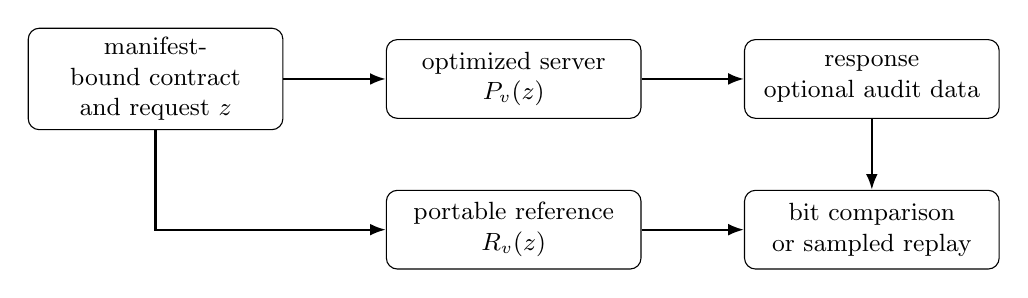
\begin{tikzpicture}[
  node distance=9mm and 13mm,
  box/.style={draw,rounded corners,align=center,text width=30mm,minimum height=10mm,font=\small},
  arr/.style={-{Latex[length=2mm]},thick}
]
\node[box] (input) {manifest-bound contract\\and request $z$};
\node[box,right=of input] (server) {optimized server\\$P_v(z)$};
\node[box,below=of server] (reference) {portable reference\\$R_v(z)$};
\node[box,right=of server] (output) {response\\optional audit data};
\node[box,right=of reference] (check) {bit comparison\\or sampled replay};
\draw[arr] (input) -- (server);
\draw[arr] (input) |- (reference);
\draw[arr] (server) -- (output);
\draw[arr] (output) -- (check);
\draw[arr] (reference) -- (check);
\end{tikzpicture}
\caption{The production execution path and its portable reference consume the same versioned
inputs.  Ordinary serving returns the response; an auditable execution additionally binds
disclosed rows before the verifier compares them.}
\label{fig:overview}
\end{figure}

Preparation transforms a supported checkpoint once, evaluates quality and implementation
gates, and emits a manifest containing the exact constants, hashes, contract version,
hardware envelope and a deterministic probe.  Serving loads those constants, refuses an
incompatible environment and evaluates $P_v$.  Verification operates at three levels:
reproduce the startup probe, replay directly disclosed intermediate rows, or authenticate and
replay rows selected after a commitment.  Table~\ref{tab:assurance} states what each
mechanism establishes.

\begin{table}[ht]
\centering
\footnotesize
\begin{tabular}{
  >{\raggedright\arraybackslash}p{0.16\textwidth}
  >{\raggedright\arraybackslash}p{0.23\textwidth}
  >{\raggedright\arraybackslash}p{0.29\textwidth}
  >{\raggedright\arraybackslash}p{0.14\textwidth}}
\toprule
Mechanism & Establishes & Does not establish & Status \\
\midrule
Contract and test vectors & A public arithmetic relation and known examples & Correctness of an arbitrary implementation or request & Implemented \\
\addlinespace[0.30em]
Kernel/reference gates & Agreement on exercised cases and negative controls & Agreement on untested inputs & Implemented \\
\addlinespace[0.30em]
Cross-architecture kit & The same source yields the same digests on every tested device & Devices not tested & Implemented \\
\addlinespace[0.30em]
Mechanized contract core & Executable bit-level LSSA semantics; sound plan, trace and audit checkers & Python or CUDA refinement; cryptographic security & Built; bridge-checked \\
\addlinespace[0.30em]
Manifest hashes & Identity of loaded files and tensor encodings & That the provider evaluated them & Implemented \\
\addlinespace[0.30em]
Startup fingerprint & Equality for one prepared probe & Execution of a later request & Implemented \\
\addlinespace[0.30em]
Authenticated row replay & Correctness of each opened row & Correctness of unopened rows & Direct replay implemented \\
\addlinespace[0.30em]
Post-commitment sampling & Detection probability in Equation~\eqref{eq:detection} & Certainty outside the sample or session binding & Primitives gated; integration disabled \\
\addlinespace[0.30em]
Interpreter as specification, signed root & A total function and a claim verifiable without the operator & --- & Planned (Section~\ref{sec:nextsteps}) \\
\addlinespace[0.30em]
Succinct or zero-knowledge proof & Full proved relation under cryptographic assumptions & --- & Not provided \\
\bottomrule
\end{tabular}
\caption{Assurance ladder.  Each mechanism adds evidence but has a deliberately limited
claim.}
\label{tab:assurance}
\end{table}
\FloatBarrier

\section{Model and Preliminaries}
\label{sec:model}

Let $T$ be sequence length, $H$ the number of query heads, $H_{kv}$ the number of key/value
heads and $d=128$ the head dimension.  Grouped-query attention maps query head $h$ to
$g(h)=\lfloor h/(H/H_{kv})\rfloor$.  Conventional causal attention for query row $i$ is
\begin{equation}
  y_{h,i}=\sum_{j=0}^{i}
  \frac{\exp(\langle q_{h,i},k_{g(h),j}\rangle/\sqrt d)}
       {\sum_{r=0}^{i}\exp(\langle q_{h,i},k_{g(h),r}\rangle/\sqrt d)}
  v_{g(h),j},
  \label{eq:softmax}
\end{equation}
which leaves evaluation order and rounding unspecified.

\begin{Def}[Contract arithmetic]
\label{def:arithmetic}
$\fl(x)$ is the result of one IEEE-754 binary32 operation in round-to-nearest,
ties-to-even mode.  $\bfround(x)$ is one round-to-nearest-even conversion from binary32 to
bfloat16.  Written products, sums and quotients are separate operations: contraction into an
FMA, reassociation, approximate division, TF32 substitution and flush-to-zero are not
permitted unless a contract clause defines them.  Integer operations are mathematical
operations followed by the explicitly stated bounded representation.
\end{Def}

The function $\rescale(x,D)$ is deliberately not a multiplication.  For $D\geq 0$ it
subtracts $D$ from the biased exponent field of a normal binary32 value while preserving sign
and significand; if $x=0$ or the resulting biased exponent would be less than one it returns
positive zero.  This avoids an underflow ambiguity found when compiling FlashAttention with
fast-math: multiplication by $2^{-D}$ may round a subnormal intermediate up to the smallest
normal, while an implementation that flushes before rounding returns zero.

\begin{Ass}[Execution platform]
\label{ass:platform}
A compliant platform provides exact two's-complement integer operations within the proven
bounds, correctly rounded binary32 arithmetic, square root and division, integer conversion,
round-to-nearest-even bfloat16 conversion and the bitwise access needed by $\rescale$.
Inputs are finite values in the contract envelope.
\end{Ass}

\paragraph{Deployment and adversary model.}
The checkpoint and contract are public.  Preparation produces a manifest with transformed
constants, their hashes, a contract version, hardware and tensor-parallel constraints and a
deterministic probe.  A provider may run arbitrary software and may attempt to return an
output without evaluating the declared model.  Hash functions are collision resistant.  For
sampled auditing the provider commits to row transcripts before learning the sample.  We
distinguish artifact integrity (files match digests), configuration conformance (the live
engine reproduces the probe) and request conformance (committed rows of a request satisfy the
contract when opened and replayed); only the third speaks about a particular request.

\section{Lockstep Softmax Attention}
\label{sec:lssa}

\subsection{Algorithmic overview}
\label{sec:lssa-overview}

LSSA-B8 replaces one conventional softmax row with six explicit stages: partition the visible
keys into fixed 128-key \emph{semantic blocks}; quantize the query and each key/value block
onto bounded power-of-two integer lattices; compute every score as an exact int32 dot
product; subtract the block maximum and map the integer distance through a public 8-bit
exponential table; accumulate the weighted values and weight sum exactly inside the block;
combine block states in ascending order through a two-level binary32 recurrence, then divide
and round once to bfloat16.

\begin{center}
\fbox{\begin{minipage}{0.90\textwidth}
\textbf{Scheduling invariant.}
An implementation may retile or reassociate work that remains inside a proved bounded
integer sum.  It may not change the semantic block partition or the order in which block
states enter the binary32 recurrence.  Parallelism is flexible where arithmetic is
associative and fixed where finite-precision addition is not.
\end{minipage}}
\end{center}

\subsection{Blockwise power-of-two quantization}

Absolute key positions are partitioned into blocks
$\mathcal{B}_b=\{128b,\ldots,\min(128(b+1),T)-1\}$.  The partition is semantic, not a kernel
tile.  A published offset $\mu_{\lambda,g,c}\in\Fth$ is subtracted from key channel $c$ at
layer $\lambda$ and KV head $g$; in ideal softmax this changes every score in a row by the
same constant and leaves Equation~\eqref{eq:softmax} unchanged, and in LSSA it acts as a
quality-improving preconditioner before quantization.

For a finite vector $x$ and a signed $p$-bit magnitude limit $L_p=2^p-1$, let
$M=\max_c|x_c|$.  If $M=0$ set $e=0$; otherwise write $M=m2^E$ with $m\in[1/2,1)$, set
$e_0=p-E$, decrement $e_0$ if $\fl(M2^{e_0})>L_p$, clamp $e$ to the operator's range and set
\begin{equation}
  Q_{p,e}(x_c)=\operatorname{clamp}_{[-L_p,L_p]}
  \left(\rne\left(\fl(x_c2^e)\right)\right).
  \label{eq:quant}
\end{equation}
For attention $p=7$ and $e\in[-32,40]$.  Queries use one exponent $e_q[h,i]$ per row and
head; keys and values use $e_k[b,g]$ and $e_v[b,g]$ over every visible row and channel of
their absolute block.  Complete blocks are append-only.  Define
\begin{equation}
  S_{i,j}=\sum_{c=0}^{d-1}q_8[h,i,c]\,k_8[g(h),j,c].
  \label{eq:score}
\end{equation}
With $s=\operatorname{clamp}(e_q+e_k,-7,23)$, $G_0=\rne(2^{26}/(\sqrt d\ln 2))$ and
\begin{equation}
  G(s)=\operatorname{clamp}_{[1,2^{30}]}
  \begin{cases}
    (G_0+\mathbf{1}_{s>0}2^{s-1})\mathbin{\texttt{>>}}s,&s\geq0,\\
    G_0\mathbin{\texttt{<<}}(-s),&s<0,
  \end{cases}
  \label{eq:gfold}
\end{equation}
all shifts and clamps are integer operations.

\subsection{The exponential table}

Let $B=26$, $n=7$, $W=9$ and $\mathsf{TOP}=255$.  The versioned table
$\mathsf{T2}\in\{0,\ldots,255\}^{17\cdot2^n}$ is
$\mathsf{T2}[k]=\operatorname{RN}_{\mathrm{half\mbox{-}up}}(255\cdot2^{-k/2^n})$ for
$0\leq k<W2^n$ and $0$ above, generated with 40-digit decimal arithmetic; its 2,176-byte CSV
SHA-256 digest is
\texttt{7a42a785940f557d5d5a4188fa5683ea00cf8b29e8d5213c75c581a5a0d92fbb}.  The ninth
doubling is maximal: rounding $255\cdot2^{-x}$ to an unsigned byte is zero for
$x>\log_2 510$.

For query row $i$ and visible block $b$,
\begin{align}
  m_b &= \max_{j\in\mathcal{B}_b,\,j\leq i} S_{i,j},\qquad
  N_b = 2^B\left\lceil\frac{m_bG(e_q+e_k)}{2^B}\right\rceil,\\
  d_j &= N_b-S_{i,j}G(e_q+e_k),\qquad
  w_j = \mathsf{T2}\!\left[\min\left(d_j\mathbin{\texttt{>>}}(B-n),2175\right)\right],
  \label{eq:weights}
\end{align}
masked keys have $w_j=0$, and the block contributes exact integer partials
\begin{equation}
  A_b[c]=\sum_{j\in\mathcal{B}_b}w_jv_8[g,j,c],\qquad
  \ell_b=\sum_{j\in\mathcal{B}_b}w_j.
  \label{eq:partials}
\end{equation}

\begin{Prop}[Integer safety and intra-block schedule invariance]
\label{prop:bounds}
For $d=128$ and block size 128, $|S_{i,j}|\leq128\cdot127^2<2^{21}$,
$|A_b[c]|\leq255\cdot127\cdot128<2^{22}$ and $0\leq\ell_b\leq255\cdot128$.  Scores and
partials fit in int32 and are exactly representable in binary32, so any reassociation or
tiling of the integer sums inside a block returns the same partials.
\end{Prop}

\begin{proof}
Each bound is the triangle inequality over a fixed number of terms with declared operand
ranges; all lie below the signed int32 limit and below $2^{24}$.  Integer addition and
multiplication are exact within these bounds, so associativity holds without overflow.
\end{proof}

\subsection{Committed two-level fold}

Blocks are grouped into segments of 32 consecutive absolute blocks (4,096 keys).  Within a
segment, visible blocks are visited in ascending absolute order with a vector $O\in\Fth^d$,
scalar $\ell\in\Fth$ and integer baseline $N$.  The first visible block initializes $N=N_b$
and $O=\ell=0$.  Before a later block, $D=(N_b-N)/2^B$ is an integer; if $D>0$ replace
$(O,\ell,N)$ with $(\rescale(O,D),\rescale(\ell,D),N_b)$ and set $r=0$, otherwise $r=-D$.  A
block with $r>32$ contributes exactly zero.  Every other block updates
\begin{align}
 O &\leftarrow \fl\!\left(O+\fl\!\left(\operatorname{float32}(A_b)2^{-(r+e_v[b,g])}\right)\right),\qquad
 \ell \leftarrow \fl\!\left(\ell+\fl\!\left(\operatorname{float32}(\ell_b)2^{-r}\right)\right).
 \label{eq:blockfold}
\end{align}
Completed segments $(O_s,\ell_s,N_s)$ are folded into the row state in ascending segment
order by the same baseline comparison, an older segment being aligned by $\rescale$ before
the explicit binary32 add.  If the final denominator is zero the output is the zero row;
otherwise $y_{h,i}=\bfround(\fl(O_{row}/\ell_{row}))$ with one correctly rounded division.

\begin{Prop}[Aligned chunk invariance]
\label{prop:chunk}
Splitting prompt ingestion only at multiples of 128 does not change any completed block's
quantized lattice, block partial or location in the committed fold, hence not the row output
whenever both executions expose the same visible prefix and row role.  A split inside a
block is not covered.
\end{Prop}

\begin{Prop}[Split-KV equivalence]
\label{prop:split}
If each segment partial is computed by the exact within-segment recurrence and the partials
are combined by the ascending outer recurrence, assigning a segment's work to any positive
number of CTAs does not change the output.
\end{Prop}

\begin{Thm}[Cross-platform bit reproducibility]
\label{thm:determinism}
Under Assumption~\ref{ass:platform}, LSSA-B8 is a deterministic map from the bit strings of
$q,k,v,\mu$, masks and contract constants to a bfloat16 output bit string; any two compliant
implementations return identical bits.
\end{Thm}

\begin{proof}
The block partition and exponent selectors are deterministic functions of the inputs;
Equation~\eqref{eq:quant} has fixed rounding and clamps; scores, maxima, shifts, table
indices and partials are exact bounded integers; the table is fixed by value and digest;
each fold transition is a specified bit-field transformation or one correctly rounded
binary32 operation with an explicit operand order.  Induction through the ascending block and
segment recurrences gives identical state bits after every transition, and the final
division and conversion are fixed.
\end{proof}

\begin{Rem}[Committed order]
Theorem~\ref{thm:determinism} does not permit a different cross-block walk:
FlashAttention-3's native descending causal traversal computes a different function.  The
gate suite includes a descending-walk negative control to ensure the comparison detects this
substitution.  Two KV-cache variants are declared as addenda: B9.1 gives absolute position
zero its own value exponent, and B9.3 gives every key its own power-of-two value grid with the
weight compensated in the fold under a per-model rounding; both keep the fold.
\end{Rem}

\section{The Complete Dense Decoder Contract (version 2.6)}
\label{sec:decoder}

Exact attention followed by conventional decoder layers would lose reproducibility.  Contract
2.6 fixes every arithmetic-bearing operation of a dense Llama-like decoder; earlier versions
differ only in the norm rule (2.5's integer norm remains selectable) and in the outlier and
smoothing folds they admit.

\subsection{Linear layers and the outlier side path}

For activation row $x\in\Fth^K$, $a_x=\fl(\max(\max_k|x_k|,10^{-8})/127)$ and
$x_8[k]=\operatorname{clamp}_{[-127,127]}\rne(\fl(x_k/a_x))$; for each output channel of a
published bfloat16 weight $W$, $a_W[n]$ and $W_8[n,k]$ are formed the same way at
preparation.  The GEMM accumulator is exact int32 and its epilogue is
\begin{equation}
 y[m,n]=\bfround\!\left(\fl\!\left(\fl(\operatorname{float32}(acc[m,n])\,a_W[n])\,a_x[m]\right)\right),
 \label{eq:linear}
\end{equation}
with a bias added as a second rounded operation.  Weight scale first is normative: it is the
order the Hopper CUTLASS scaled-int8 epilogue reproduces, and swapping the scales is a
different function.  Contract 2.5 adds a declared outlier side path: for each linear a
manifest-listed set of up to eight input channels is excluded from the int8 product and
re-added through a separate bf16 product in a declared order, which removes the
per-channel outliers that otherwise force the int8 grid to lose resolution.

\subsection{The float RMSNorm (2.6) and the integer RMSNorm (2.5)}

Contract 2.5 quantizes a row onto a signed 15-bit power-of-two grid, forms the sum of squares
and the scaled $N\epsilon$ term exactly in int64, and indexes a published reciprocal
square-root table; carrying $\epsilon$ is essential, since omitting it over-normalizes
low-energy embedding rows in models such as Mistral.  Contract 2.6 replaces the table by an
fp32 rule with an index-pinned reduction: squares $\fl(x_jx_j)$, chains of eight in element
order, an adjacent-pairs balanced tree over the chains (splitting at the largest power of two
below the count), $S'=\fl(S+\fl(N\epsilon))$, $S''=\max(S',2^{-126})$,
$rs=\fl(\sqrt N/\fl(\sqrt{S''}))$ with one IEEE square root and one IEEE division, and
$\bfround(\fl(\fl(x_jrs)\,g_j))$.  The tree is defined by element index alone so a 32-lane
warp, a 64-lane wavefront and a CPU reproduce the same additions; the reciprocal square root
is not a transcendental but two operations IEEE-754 requires to be correctly rounded.  Both
rules are gated bit-identical to their references; 2.6 is the served default because it
removes a table and is faster on models with per-head query/key norms (Section~\ref{sec:eval-perf}),
and 2.5 stays selectable for proof systems that prefer integer-only arithmetic.

\subsection{Rotary embeddings, SiLU, rotations, smoothing}

Rotary embeddings use a manifest-published Q14 table; for a rotary pair $(t_1,t_2)$ with
table row $(c,s)$, $t'_1=\bfround(\fl(\fl(t_1c)-\fl(t_2s)))$ and
$t'_2=\bfround(\fl(\fl(t_2c)+\fl(t_1s)))$ without contraction.  SiLU is a ten-step binary32
program over a frozen 8,192-entry integer table with one bfloat16 rounding.  Orthogonal
Hadamard transforms flatten outliers before quantization: offline R1 changes the residual
basis by folding into embedding, head and adjacent weights, R2 rotates the value/output head
dimension, and online R4 applies an eight-stage Sylvester butterfly to each 256-lane block
before the down projection, every add/subtract a separate binary32 operation followed by an
exact $2^{-4}$ scale.  R1 online keeps the residual stream in the original basis and rotates
the normalized output immediately before quantization.  A SmoothQuant-like per-channel scale
\cite{xiao2023smoothquant} can be folded into adjacent constants; its selected scale and fold
level are hashed manifest constants.

\subsection{Head and tensor parallelism}

The language-model head quantizes activations and weights to 15-bit magnitudes split into two
int8 planes; four int32 GEMMs are combined exactly in int64 before the variant's declared
scale order and bfloat16 conversion.  For tensor-parallel world size $P$, row-parallel
partials are reduced as $y=\bfround(\fl(\fl(y_0+y_1)+\cdots+y_{P-1}))$ in increasing rank
order with one final rounding; an all-gather with a local fold or a column-block all-to-all
may implement it, but NCCL's unconstrained reduction order is not the contract.

\section{The Mixture-of-Experts Contract (version 3)}
\label{sec:moe}

A routed feed-forward block adds three operations that a dense contract does not have: a
gate that scores tokens against experts, a top-$k$ selection with normalization, and a
weighted combine of per-expert outputs.  Each is a place where an engine's implementation
choice (fp32 versus bf16 logits, softmax library, tie handling, accumulation order across
experts) changes bits.  Contract v3 fixes all three and reuses the dense contract for the
expert matmuls.

\subsection{Gate, router, combine}

The gate is an int8 linear under Equation~\eqref{eq:linear} on the block input (a bias, if
the model has one, is added as a rounded operation).  Router scores are integers: with $g$
the gate output and $m$ its row maximum,
\begin{equation}
  d=\rne\!\left(\fl(m-g)\cdot\fl(2^{26}/\ln 2)\right),\qquad
  s=\mathsf{TAB}[(d\mathbin{\texttt{>>}}13)\,\&\,8191]\mathbin{\texttt{>>}}(d\mathbin{\texttt{>>}}26),
\end{equation}
where $\mathsf{TAB}$ is the SiLU contract's 8,192-entry table, so $s$ is a monotone integer
proxy for $\exp(g-m)$ on a public lattice.  Top-$k$ selects the $k$ largest $s$ with ties
broken to the lowest expert index; with $S$ the sum of the selected scores the routing
weights are $w_e=\bfround(\fl(s_e)/\fl(S))$ (or the raw scores' normalization when the model
does not renormalize).  Dispatch is a stable sort of tokens by expert: a permutation, exact.
Each expert applies the dense contract's SwiGLU block (two int8 linears, the table SiLU, the
R1 or R4 rotation on the down input, the third linear).  The combine accumulates
$\bfround(\fl(w_e\cdot y_e))$ for the token's selected experts in ascending expert index in
binary32 with one final bfloat16 rounding.  Experts' outputs can therefore be computed by any
grouped kernel, in any order, on any tile shape; only the per-token fold order is fixed.

\subsection{Addendum: GPT-OSS}

GPT-OSS \cite{gptoss2025} adds a gate bias, expert biases and a clamped, gated SiLU:
$g_c=\min(g,7)$, $u_c=\operatorname{clamp}(u,-7,7)$,
$\mathrm{glu}=\bfround(g_c\cdot\sigma(\bfround(1.702\,g_c)))$ with the SiLU table's sigmoid,
$h=\bfround((u_c+1)\cdot\mathrm{glu})$; the checkpoint's interleaved gate/up rows are
de-interleaved at fold time; and because its hidden and intermediate widths (2,880) are not
multiples of 256 the rotation is declared on 64-lane blocks or omitted.  All of these are
manifest fields, not engine defaults.

\subsection{Consuming MXFP4 weights exactly}
\label{sec:mx}

GPT-OSS ships its expert weights in the microscaling format \cite{mxfp4}: E2M1 values in
blocks of 32 with a shared E8M0 exponent.  Requantizing such weights to int8 per-channel
scales is one admissible route (Section~\ref{sec:parity}).  The second route consumes the
published bits directly.  Let $x_8$ be the int8 activation row, $m_j\in\{0,\pm1,\ldots,\pm6\}$
the doubled E2M1 mantissas of block $b$ and $k_b$ its exponent byte.  The contract declares
\begin{equation}
  s_b=\sum_{j\in b}x_8[j]\,m_j\ \text{(exact int32)},\qquad
  acc\leftarrow\fl\!\left(acc+\fl(s_b)\cdot2^{k_b-128}\right)\ \text{in ascending }b,
  \label{eq:mx}
\end{equation}
and the epilogue $\bfround(\bfround(acc\cdot a_x)+\beta)$.  Because $|s_b|\leq32\cdot127\cdot
12<2^{22}$, $\fl(s_b)$ is exact and the product with a power of two is exact, so the only
rounding per block is the one addition; the rule is a total function of the checkpoint bytes
and the activations.  A power of two is formed by bit construction, never by a
transcendental.  This is the route served in Section~\ref{sec:eval-moe}; its cost is
analysed in Section~\ref{sec:parity}.

\section{Implementation}
\label{sec:system}

\subsection{Preparation, manifest, serving, refusal}

Preparation validates the model envelope before GPU work (architecture, dimensions, head
size, sliding-window rules, context, tensor-parallel world size); calibrates or imports the
per-layer key offset and optional smoothing statistics; loads a vLLM engine on the
transformation path, folds rotations and gains, quantizes weights and exports constants from
each worker; runs a deterministic 256-token probe twice and refuses a non-self-consistent
result; runs per-operator identity, stock-log-probability, fused-kernel and whole-stack
perplexity gates; and hashes every file and tensor into a manifest that is read back and
verified.  A tensor digest includes a domain tag, dtype, shape and raw little-endian bytes.
With the manifest set, each vLLM process validates it, resolves a configuration from the GPU
and topology, registers the custom attention backend and arms the full stack from the
exported constants; strict mode refuses a hardware class that cannot reproduce the manifest,
a different world size, a context mismatch, an unarmed layer class or any digest failure.  The
guarded server replays the probe through the OpenAI-compatible endpoint, comparing each
prompt token's log-probability bits and eight greedy token identifiers, and dies on mismatch.
A scheduler hook enforces 128-aligned prefill chunks (Proposition~\ref{prop:chunk}).

\subsection{Attention and dense kernels}

Prompt rows execute in a modified FlashAttention-3 kernel: int8 WGMMA forms exact int32
scores, the block-local maximum and table lookup operate on the score tile, integer PV forms
$A_b$, and the epilogue executes the ascending two-level fold; the build disables
flush-to-zero and uses correctly rounded division.  Generated rows use a paged split-KV
kernel over the same append-only lattice with two eight-warp groups alternating blocks inside
one CTA.  The non-attention stack registers opaque CUDA operations so graph compilation
cannot decompose or reassociate them; fused consumers combine normalization, quantization,
linear epilogues, RoPE, SiLU, the outlier side path and R4 where the contract permits, and
Qwen3's per-head query/key norm is fused into the projection epilogue under the 2.6 rule.
Small-row GEMMs use \texttt{torch.\_int\_mm}; larger rows use the Hopper CUTLASS scaled-int8
path; both are gated against the declared epilogue.

\subsection{Mixture-of-experts kernels}

The MoE block is armed at model load, before graph capture, by replacing vLLM's fused-MoE
forward.  One kernel computes the int8 gate (interleaved 32-byte weight reads), the table
scores and the top-$k$ with the tie rule, and optionally the R1-rotated row quantization, for
batches up to 512 tokens; a 1,024-thread dispatch performs the counting sort and row copy; the
expert matmuls run on a CUTLASS grouped int8 GEMM at large batches and on an exact GEMV form
at few rows (the grouped kernel schedules a full wave of CTAs over eight one-row problems and
loses); a multi-row grouped epilogue applies the activation, the rotation and the requantization
one warp per 256-lane block; and a block-per-token kernel folds the combine.  For the
MXFP4-consuming rule the operand is unpacked from nibbles to int8 in registers with a
negative-zero mask, per-block partials come from int8 tensor-core \texttt{mma.sync}
instructions at 32-wide $K$ so that each instruction is exactly one block, and the rounded
update of Equation~\eqref{eq:mx} follows each; the decode tile is a warp-specialized 16-row
form with four producer warps loading and unpacking into a three-deep ring and eight consumer
warps computing.  The exact magic-number integer-to-float conversion
($\fl(\mathrm{bits}(s+3\cdot2^{22})-1.5\cdot2^{23})$, exact for $|s|<2^{22}$) replaces the
quarter-rate conversion instruction; it changed nothing in time, which located the cost
elsewhere (Section~\ref{sec:parity}).

\section{Verification and Audit Protocol}
\label{sec:audit}

\subsection{Oracle hierarchy and cross-architecture kit}

The implementation uses a one-way hierarchy: the normative contract defines constants,
domains, order, masks, roundings and refusals; a scalar golden in Python integers and
explicit binary32 operations implements the text; a torch reference vectorizes independent
rows but keeps the sequential fold; standalone kernels compare output bits to the reference
across shapes, splits and negative controls; the live engine dumps rows and lattice state
for the reference to reconstruct; the manifest and probe bind constants and reject a
deployment whose fingerprint differs.  A gate failure is repaired in the optimized
implementation; the oracle is never widened.  Negative controls (a descending block walk, a
non-aligned chunk cut, truncation in the table, approximate division, multiplication-based
rescaling, tampered constants) must differ.

A cross-architecture kit fixes inputs by a seeded generator with tie-dense and edge rows
(zero rows, single-spike rows, $10^{-30}$ and $10^{-19}$ scale rows), builds the kernel
sources for the local GPU, checks every kernel against its torch reference and its numpy twin
on that machine, and writes the SHA-256 of every output.  Identical digests on two machines
are bit-identical results.  Running it taught one rule: a record is only evidence if it was
produced by the committed kit on the committed inputs; two records in the repository predated
later edits of their kits and did not reproduce until regenerated, while the arithmetic held
on every machine.

\subsection{Mechanized contract core}
\label{sec:lean}

The contract core is mechanized in Lean~4.33.1 \cite{demoura2015lean} (the third author's
contribution).  The development is deliberately narrower than a
verification of the deployed CUDA program: it proves properties of the formal model and
exports artifacts that an independent Python bridge recomputes.  Its structural theorems
keep the LSSA fold parameterized by a small deterministic rounding interface, isolating the
operations at which finite-precision order matters, and then instantiate that interface over
bit vectors: exact dyadic decoding and integer rounding define finite binary32 addition and
division, exponent-field rescaling and bfloat16 conversion, and a concrete quantized-row
evaluator produces all 128 bfloat16 output channels of a row.  Determinism
(\texttt{lssa\_deterministic}) and legal schedule refinement
(\texttt{scheduled\_refines\_canonical}, \texttt{splitKV\_refines\_canonical}) hold inside
this model; Assumption~\ref{ass:platform} and the gates connect its words and operation
order to hardware.

\begin{table}[ht]
\centering
\footnotesize
\begin{tabular}{>{\raggedright\arraybackslash}p{0.17\textwidth}>{\raggedright\arraybackslash}p{0.41\textwidth}>{\raggedright\arraybackslash}p{0.30\textwidth}}
\toprule
Layer & Representative checked declarations & Connected artifact or gate \\
\midrule
Concrete numeric semantics & \texttt{addRNE}, \texttt{divideRNE}, \texttt{toBF16RNE}, \texttt{rescale\_subtracts\_exponent}, \texttt{single\_token\_row\_vector} & binary32 operations, bfloat16 ties, rescale cases, a complete 128-channel row vector \\
\addlinespace[0.35em]
LSSA and runtime plans & \texttt{score\_abs\_le}, \texttt{lssa\_deterministic}, \texttt{scheduled\_refines\_canonical}, \texttt{splitKV\_refines\_canonical}, \texttt{check\_segment\_plan\_sound} & integer bounds, T2 anchors, chunking, split-KV, fail-closed schedule gates \\
\addlinespace[0.35em]
Decoder and admission & \texttt{validateParams\_sound}, \texttt{linear\_acc\_abs\_lt}, \texttt{rmsnorm\_sum\_lt\_int64}, \texttt{head\_recomposition\_lt\_int64} & pinned model envelope, decoder bounds (the 2.5 integer norm), tensor-parallel order \\
\addlinespace[0.35em]
Authenticated evidence & \texttt{row\_encoding\_injective}, \texttt{manifest\_validation\_sound}, \texttt{check\_trace\_sound}, \texttt{check\_openings\_sound} & typed transcript preimages, fail-closed manifests, trace chains, Merkle openings \\
\addlinespace[0.35em]
Audit and approximation & \texttt{detection\_certain\_when\_sample\_exceeds\_valid\_rows}, \texttt{local\_attention\_error\_bound}, \texttt{fidelity\_certificate\_sound} & sampling counts and a local error certificate; no model-quality theorem \\
\addlinespace[0.35em]
Logical GPU layout & \texttt{score\_term\_coverage}, \texttt{row\_head\_channel\_disjoint}, \texttt{cta\_segment\_coverage} & machine-readable logical obligations plus explicit hardware assumptions \\
\bottomrule
\end{tabular}
\caption{Mechanized statements and their implementation bridge.  Declaration names identify
the Lean definitions and proof objects; a passing runtime gate is evidence of implementation
agreement, not a replacement for those proofs.}
\label{tab:lean}
\end{table}

The tree contains no admitted theorem or project-specific axiom.  The executable
\texttt{lockstep-formal} exports a deterministic artifact with the contract constants and
table digest, numeric and full-row vectors, negative witnesses, audit and fidelity examples
and logical GPU obligations; the Python bridge regenerates the decimal T2 table and the
corresponding values, compares the complete object, and includes a mutation test that must
reject a changed digest.  The trusted boundary is explicit: SHA-256 and BLAKE3 collision
resistance, CUDA memory and WGMMA instruction semantics, compiler lowering, PTX/SASS binary32
behaviour, the Python/Torch runtime and the source-to-machine-code relation are assumptions
or tested links, not theorems.  Two gaps are scheduled: the decoder theorems bound the 2.5
integer norm and need the 2.6 float norm (a correctly rounded square root in the binary32
model), and the mixture-of-experts contract is not yet in the development
(Section~\ref{sec:nextsteps}).

\subsection{Fingerprint and committed sampled replay}

The fingerprint is the ordered vector of bfloat16 prompt-log-probability bits and greedy
token identifiers produced during preparation; a successful live check establishes
$F_{\mathrm{live}}(p)=F_M(p)$ for that probe, and hash verification that the live constants
equal the manifest's.  For an auditable request the leaf packer serializes every attention
head's $q,k,v,o$ row plus one exponent byte per head ($2(H+H_{kv})(d+1)$ bytes, 8,256 for
Qwen2.5-7B); keyed BLAKE3 hashes each leaf and a binary parent tree.

\begin{Prot}[Post-commitment row audit]
\label{prot:audit}
For a request with $N$ auditable layer--row leaves: the provider computes the inference,
forms canonical leaves and sends a binding root; an independent beacon or verifier challenge
then selects $s$ distinct indices; the provider reveals each selected leaf, its
authentication path and the prefix state the reference needs; the verifier authenticates the
opening, reconstructs the lattice, evaluates the contract and compares bits.
\end{Prot}

\begin{Prop}[Sampling detection probability]
\label{prop:sampling}
If the commitment is binding and the sample is uniform without replacement after the root is
fixed, and exactly $c$ of $N$ rows are invalid, Protocol~\ref{prot:audit} detects at least one
with probability
\begin{equation}
  1-\binom{N-c}{s}\Big/\binom{N}{s}.
  \label{eq:detection}
\end{equation}
\end{Prop}

A valid opening with a differing bit is a compact certificate of nonconformance.  The
protocol does not imply unselected rows are correct, does not hide model or prompt data, and
needs a session-binding protocol to attribute a response to a client.  The prototype's key is
fixed and supplies domain separation, not authentication; Section~\ref{sec:nextsteps}
replaces it with a signature.

\section{Evaluation}
\label{sec:evaluation}

\subsection{Methodology}

The baseline is stock vLLM 0.25.1 with bf16 weights and FlashAttention-3.  Lockstep and stock
runs use the same node and session, one process per stack, \texttt{FULL\_AND\_PIECEWISE}
CUDA graphs, inductor disabled, prefix caching off.  Throughput ratios are Lockstep divided by
stock; TTFT ratios are stock time divided by Lockstep time, so larger is better in both cases.
The serving device is one NVIDIA H100 80GB unless stated; Qwen2.5-72B uses four at tensor
parallelism four.  Single-stream cells are medians of three matched measurements; the stock
arm of the 7B was repeated after the Lockstep arm and agreed within half a percent.  Served
rows use \texttt{vllm bench serve} with 64 concurrent requests on ShareGPT prompts
(workload W1; W2 mixed and W3 prefill-heavy are stated where used), 500 prompts, three
repetitions per arm for the MoE rows.  Quality is the percentage change in wikitext-2
perplexity against the same model on stock vLLM on the same node (30 windows for the
acceptance gate; 300 windows with a paired bootstrap where stated), and for GPT-OSS, a chat
model whose harmony format makes raw wikitext invalid, chat-templated ShareGPT conversations
at 2,048 tokens.  Every number below carries its date; all were measured between 2 and 10
September 2026 and the raw logs and result files are retained in the artifact.  This is a
single-node, eight-day campaign: cells have no confidence intervals unless stated.

\subsection{RQ1: Implementation agreement}

\textbf{Answer.}  Every exercised comparison returned zero differing bits, from scalar
definitions through live prompt, decode, fused-stack, tensor-parallel and MoE boundaries.

\begin{table}[H]
\centering
\small
\begin{tabular}{>{\raggedright\arraybackslash}p{0.30\textwidth}>{\raggedright\arraybackslash}p{0.55\textwidth}r}
\toprule
Boundary & Coverage & Differences \\
\midrule
Python golden $\leftrightarrow$ torch attention & 28 checks, 119 constructed/random cases (B8); 239 (B); 176 (B9) & 0 \\
Torch $\leftrightarrow$ decode kernels & 21 shape families, sink on and off; K1--K8 43 cases; K9 10 & 0 \\
Long split-KV control & split 64 vs.\ split 1 at 262K, 512K and 1M keys & 0 \\
Engine prompt rows (E1) & 151,200 (Qwen2.5-7B), 172,800 (Llama-3.1-8B), 86,400 (Llama-3.1-70B, TP=4) & 0 \\
Engine generated rows (E4) & 29,736 (7B); token identity across batch compositions and permutations (F3) & 0 \\
Verifier replay of an H100 dump & 370,020 prompt and 2,352 generated rows on RTX 4090 and Apple M4 Max, a 168-row generated sample on x86, all rows on B200 (SPEC 7.18, 7.21) & 0 \\
Declared $\leftrightarrow$ fused dense stack & 1,186 kernel cases on captured real activations & 0 \\
Float norm 2.6 & 160 cases, kernel = torch = numpy; R4 quantiser 48; fused head norm 48 (S26G) & 0 \\
Tensor-parallel reduction & 32 custom-all-reduce cases vs.\ rank fold & 0 \\
MoE kernels & route 60, combine 20, dispatch 18, grouped GEMM 64, epilogues 8--20 (263 cases); MX GEMV 10, MX tile identity 5 forms & 0 \\
MoE engine & Qwen3-30B-A3B engine perplexity 8.81400582424298 on eight readings; GPT-OSS engine perplexity identical across kernel forms & 0 \\
Cross-architecture kit (2.6) & 158 cases, 538 output digests, H100 sm\_90 / RTX 4090 sm\_89 / RTX PRO 6000 Blackwell sm\_120 & 0 \\
CPU legs of the float norm & 72 cases, x86 (numpy 1.26, 2.3; torch 2.4, 2.11) and Apple silicon ARM (numpy 2.5) vs.\ the H100 reference digests & 0 \\
\bottomrule
\end{tabular}
\caption{Exactness gates.  Every comparison is bit equality; zero is the only passing
count.  Case counts are those of the most recent run of each gate on the merged tree.}
\label{tab:exactness}
\end{table}
\FloatBarrier

\subsection{RQ2: Serving efficiency}
\label{sec:eval-perf}

\textbf{Answer.}  On single-stream decode every measured dense family is at or above stock
at every batch; on 2K and 8K prompts every family is at or above stock; at 32K the families
are within 6\%.  The remaining gaps are 128-token prompts (a fixed per-layer cost),
saturated short-turn chat, and sub-4B models.

\begin{table}[H]
\centering
\footnotesize
\begin{tabular}{>{\raggedright\arraybackslash}p{0.24\textwidth}>{\raggedright\arraybackslash}p{0.22\textwidth}>{\raggedright\arraybackslash}p{0.24\textwidth}>{\raggedright\arraybackslash}p{0.20\textwidth}}
\toprule
Model (one H100 unless stated) & Workload points & Lockstep / stock & Reading \\
\midrule
Qwen2.5-7B & TTFT 128 / 2K / 8K / 32K & 0.90 / 1.03 / 1.06 / 0.99 & parity from 2K \\
Qwen2.5-7B & decode batch 1 / 8 / 32 & 1.14 / 1.10 / 1.01 & above stock \\
Qwen2.5-7B & served chat / mixed / prefill-heavy & 0.87 / 0.97 / 0.97 & chat: decode-kernel fixed cost at short context \\
Llama-3.1-8B & TTFT 128 / 2K / 8K / 32K; decode 1 / 8 / 32 & 0.91 / 1.04 / 1.08 / 0.99; 1.10 / 1.05 / 1.01 & parity \\
Mistral-7B & TTFT 128 / 2K / 8K / 32K; decode 1 / 8 / 32 & 0.91 / 1.05 / 1.07 / 0.97; 1.13 / 1.09 / 1.04 & parity \\
Phi-4-mini (2.5) & TTFT 128 / 2K / 8K / 32K; decode 1 / 8 / 32 & 0.97 / 1.00 / 1.04 / 0.94; 1.18 / 1.16 / 1.11 & above stock on decode \\
Phi-4-mini (2.6, second node) & TTFT 128 / 2K; decode 1 / 8 / 32 & 0.88 / 1.07; 1.23 / 1.21 / 1.13 & above stock \\
Qwen3-8B (2.5, unfused head norm) & TTFT 128 / 2K / 8K / 32K; decode 1 / 8 / 32 & 0.62 / 0.45 / 0.51 / 0.56; 0.82 / 0.82 / 0.86 & the row the 2.6 fusion fixed \\
Qwen3-8B (2.6, fused head norm, second node) & TTFT 128 / 2K / 8K; decode 1 / 8 / 32 & 0.90 / 1.10 / 1.13; 1.18 / 1.13 / 1.04 & parity from 2K \\
Qwen2.5 size sweep 1.5B / 3B / 7B / 14B & TTFT 8K; decode batch 1 & 0.78 / 0.89 / 1.06 / 1.09; 0.86 / 0.94 / 1.14 / 1.01 & fixed per-layer cost amortized by size \\
Qwen2.5-7B-1M & TTFT 32K / 65K / 131K / 262K; decode at 131K & 0.86 / 0.85 / 0.82 / 0.81; 1.15 & int8 KV: decode faster than stock \\
Qwen2.5-72B, TP=4 & served chat / mixed / prefill-heavy & 0.91 / 0.98 / 0.98 & within ten percent \\
\bottomrule
\end{tabular}
\caption{Whole-contract performance against stock vLLM.  Decode and served entries are
throughput ratios; TTFT entries invert latency so values above one are better.  Rows dated
2026-09-09 (Stage II clean re-baseline, one node, one session: SPEC 7.24--7.26 and the
\texttt{PLAN\_24} log; the size sweep from the same log), 2026-09-10 (2.6 rows, measured by
the second author on a second H100 node, both arms served from manifests,
\texttt{results/contract3\_20260910/logs26/final}), and 2026-09-06 (the 72B served row,
SPEC 7.17).}
\label{tab:performance}
\end{table}

Absolute readings anchor the ratios: on Qwen3-8B the 2.6 configuration decodes at 167.8 /
1,249 / 4,293 tokens/s against stock's 142.4 / 1,108 / 4,118, and reaches first token at 2K
in 47.8\,ms against 52.8\,ms; on Phi-4-mini 246.3 / 1,823 / 6,151 against 200.4 / 1,502 /
5,468 (medians of three, \path{results/contract3_20260910/logs26/final/TABLE.txt}).  The
7B's saturated-chat gap is the decode kernel's fixed cost per launch at one to three 128-key
blocks; its per-tile split is the filed next candidate.  The largest single item of the
campaign was not a kernel but a dead code route (a logits hook re-installed above a fused
head on second arming) that had cost every earlier measurement a per-step int64 combine over
the vocabulary; removing it took batch-32 decode from 0.85$\times$ to 1.03$\times$ on its
own.
\FloatBarrier

\subsection{RQ3: Model fidelity}

\textbf{Answer.}  Every accepted manifest is within the one-percent wikitext-2 band; the
2.6 norm changes perplexity by less than 0.04 percentage points against 2.5; and on GPT-OSS
the exact-MXFP4 route is 2.1\% better than stock's own MXFP4 path on chat text.

\begin{table}[H]
\centering
\footnotesize
\begin{tabular}{>{\raggedright\arraybackslash}p{0.20\textwidth}>{\raggedright\arraybackslash}p{0.13\textwidth}r@{\hspace{1.2em}}>{\raggedright\arraybackslash}p{0.22\textwidth}>{\raggedright\arraybackslash}p{0.08\textwidth}r}
\toprule
Family & Model & $\Delta$PPL (\%) & Family & Model & $\Delta$PPL (\%) \\
\midrule
Qwen2.5 (2.5) & 7B & +0.27 & Qwen3 (2.5 / 2.6) & 8B & $-0.31$ / $-0.39$ \\
Qwen2.5 (2.5) & 1.5B / 3B / 14B & +0.23 / +0.21 / +0.52 & Qwen3 (2.2) & 4B & $-0.26$ \\
Qwen2.5 (2.5) & 7B-1M & +0.23 & Qwen3 (2.2), TP=2 & 32B & $-0.04$ \\
Qwen2.5 (2.2), TP=2 & 32B & +0.10 & Llama-3.2 (2.5) & 3B & $-0.11$ \\
Qwen2.5 (2.5), TP=4 & 72B & +0.14 & Llama-3.1 (2.5) & 8B & +0.22 \\
Phi (2.2) & 4 (14B) & +0.12 & Llama-3.1 (2.5, B9.3), TP=4 & 70B & +0.81 \\
Phi (2.5 / 2.6) & 4-mini & +0.55 / +0.61 & Mistral (2.5) & 7B & +0.09 \\
Qwen3-30B-A3B (v3, rotations on / off) & MoE & +0.12 / +0.71 & & & \\
GPT-OSS-20B (chat; exact MXFP4 / int8 experts) & 14.790 / 15.531 vs.\ 15.101 & $-2.06$ / $+2.85$ & & & \\
\bottomrule
\end{tabular}
\caption{Whole-stack perplexity change relative to stock on the same node (wikitext-2, 30
windows of 1,024 at stride 512; the contract version in parentheses; SPEC 7.20, 7.23, 7.24,
7.27).  The 2.6 rows are 300 windows on a second node with a paired bootstrap of 2.6 against
2.5: $-0.035\%$ $[-0.105,+0.036]$ on Qwen3-8B and $+0.011\%$ $[-0.071,+0.090]$ on Phi-4-mini
(\texttt{results/contract3\_20260910/logs26}).  Rows labelled 2.2 are fingerprints of the
Stage 1 matrix not re-run under the served contract.  The 70B row is one cell of the B9.3
rounding ladder (SPEC 7.23).  Qwen3-30B-A3B uses 30 windows of 2,048.  GPT-OSS is
chat-templated ShareGPT at 2,048 tokens, 30 windows.}
\label{tab:quality}
\end{table}

The band is an admission policy, not a universal criterion: Llama-3.1-70B at TP=4 reproduces
a synthetic fingerprint but was refused under 2.4 (about $+4.9\%$) and under B9.1
($+1.77\%$); the B9.3 per-key value grid brings it to $+0.81\%$ and admits it.  The
GPT-OSS int8-expert row is outside the band, and Section~\ref{sec:parity} says why.
\FloatBarrier

\subsection{RQ4: Auditability across devices}

\textbf{Answer.}  Direct heterogeneous replay reproduces H100 rows bit for bit on Ada,
Blackwell, x86 and ARM; request commitment and sampled auditing are gated primitives, not
yet deployed.

An H100 attention dump was replayed by the reference on an RTX 4090 (all steps, 3.2\,s), its
x86 host (sampled steps, 105\,s), an Apple M4 Max (all 96 steps, 194.5\,s) and a B200
(1.8\,s), with zero differing bits.  The 2.6 kit adds Blackwell Server Edition (sm\_120) to
the GPU set and the numpy twin on x86 and ARM CPUs reproduces the H100 reference digests on
every norm case (Table~\ref{tab:exactness}).  These replays differ in workload and are
feasibility readings, not a normalized verifier-throughput comparison.  Opening $s$ rows of
Qwen2.5-7B transfers at least $8{,}256s$ bytes plus authentication paths; commitment
throughput and challenge latency are not reported because the serving integration is
disabled.

\subsection{RQ5: Coverage}

\textbf{Answer.}  Dense Llama-like decoders with head dimension 128 (Qwen2.5, Qwen3, Llama
3.x, Mistral, Phi-4) and two mixture-of-experts models (Qwen3-30B-A3B, GPT-OSS-20B), Hopper
production serving, reference replay on Ada, Blackwell, x86 and ARM, contexts through one
million tokens for selected decode tests, and tensor parallelism through four.  The envelope
refuses head dimensions other than 128, active sliding windows, multimodal and
encoder--decoder models, pre-quantized dense checkpoints and any undeclared configuration.
GPT-OSS's attention (head dimension 64, a 128-token window on alternate layers, a learned
sink logit) is therefore served by stock FlashAttention today: its MoE layers are on the
contract, its attention is not, and the manifest states so.

\subsection{RQ6: Mixture of experts}
\label{sec:eval-moe}

\textbf{Answer.}  The construction extends to routed models with no loss of exactness.  On
the int8 expert rule the MoE model serves above stock; on the exact-MXFP4 rule it serves
exactly but at about half stock's throughput, for a reason the next section makes
structural.

\begin{table}[H]
\centering
\footnotesize
\begin{tabular}{>{\raggedright\arraybackslash}p{0.22\textwidth}>{\raggedright\arraybackslash}p{0.19\textwidth}>{\raggedright\arraybackslash}p{0.13\textwidth}>{\raggedright\arraybackslash}p{0.36\textwidth}}
\toprule
Model, rule & Workload points & Lockstep / stock & Absolute (Lockstep vs.\ stock) \\
\midrule
Qwen3-30B-A3B, v3 int8 & decode batch 1 / 8 / 32 & 0.87 / 1.04 / 1.26 & 177.9 / 921.1 / 2,811.6 vs.\ 203.9 / 889.5 / 2,222.8 tok/s \\
Qwen3-30B-A3B, v3 int8 & TTFT 2K / 8K & 0.86 / 0.88 & 52.1 / 192.2 vs.\ 44.8 / 168.9 ms \\
Qwen3-30B-A3B, v3 int8 & served W1, 64 concurrent & \textbf{1.32--1.37}; TPOT 0.72 & 14.57, 14.54 req/s vs.\ 10.66, 11.06, 10.97 (stock spread 4\%); TPOT 17.3 vs.\ 23.9 ms \\
GPT-OSS-20B, exact MXFP4 & decode batch 1 / 8 / 32 & 0.62 / 0.33 / 0.32 & 190.3 / 524.2 / 1,521.2 vs.\ 309.1 / 1,574.6 / 4,833.4 tok/s \\
GPT-OSS-20B, exact MXFP4 & TTFT 2K / 8K & 0.31 / 0.32 & 107 / 376 vs.\ 36.6 / 126.6 ms \\
GPT-OSS-20B, exact MXFP4 & served W1, 64 concurrent & 0.54 (M2E6); 0.52 after the regression fix (M2E14) & 10.32 / 9.98 req/s, 2,060 / 1,991 tok/s vs.\ 19.15, 3,821 \\
GPT-OSS-20B, int8 experts (early reading, M2E2) & decode 1 / 8 / 32; TTFT 2K / 8K & 0.85 / 0.72 / 0.71; 0.80 / 0.83 & before the router, dispatch and GEMV changes that lifted Qwen3-30B's rows by 16--40\% \\
\bottomrule
\end{tabular}
\caption{Mixture-of-experts rows, one H100, 2026-09-10 (SPEC 7.27; \texttt{docs/PLAN\_3.md}
entries M1F11 with its stock arm from M1E9, M1S4/M1S5, M2E2, M2E6, M2E8, M2E9, M2S1;
\texttt{results/s3}).  Stock GPT-OSS runs vLLM's Triton MXFP4 kernels; stock Qwen3-30B runs
bf16.  The Qwen3-30B served row is three stock repetitions against two Lockstep repetitions
agreeing within 0.2\%; batch 8 decode is one reading above the line.}
\label{tab:moe}
\end{table}

The Qwen3-30B served row: the contract path is faster than stock under load
because its experts read int8 weights (half the bytes of bf16) and its grouped kernels run at
433--588 TOPS, and because the router and combine are small integer kernels; the
single-stream batch-1 gap is the fixed cost of the gate and dispatch launches at one token.
GPT-OSS's exact-MXFP4 row is slower for the reasons analysed next; its engine perplexity is
identical across every kernel form and its fused path is bit-identical to the CPU reference on
real tokens.
\FloatBarrier

\section{Reaching Parity on Mixture-of-Experts Models}
\label{sec:parity}

The contract reaches parity and above on routed models under one rule and sits below it
under another; three facts fix which is which.

\paragraph{Fact 1: the int8 expert rule is above stock today.}  Qwen3-30B-A3B serves at
1.32--1.37$\times$ stock (Table~\ref{tab:moe}) with every MoE kernel gated bit-identical and
the engine's perplexity identical across eight readings.  This is the same rule as the dense
linears, on the same kernels, and it is the rule Chen's independent measurement supports on
quality: requantizing
scales to powers of two gives byte-identical tokens across kernels at a perplexity cost of
$+0.32\%$, $-0.28\%$ and $+0.48\%$ at 1.7B, 8B and 14B \cite{chen2026pow2}, the same order
as our accepted dense rows.

\paragraph{Fact 2: the exact-MXFP4 rule has a speed floor below parity, and the floor is
arithmetic, not engineering.}  Equation~\eqref{eq:mx} requires, per 32-wide block of every
output element, an exact integer partial followed by one rounded binary32 update.  On the
tensor-core path that is one \texttt{mma.m16n8k32} instruction per block and fragment
followed by four fused multiply-adds: the fp32 side is $1/32$ of the MAC count at roughly
$1/15$ of the tensor-core rate, so the rounded update alone costs about half the matrix time,
and the nibble-to-int8 expansion is proportional to the weight bytes.  int8 weights pay
neither.  The standalone measurements at the served decode regime (256 dispatched rows over 32
experts, $N=5{,}760$, $K=2{,}880$): the int8 grouped kernel takes 0.201\,ms reading twice the
bytes, the pipelined 16-row MX tile 0.300\,ms, and the best MX form measured, a
warp-specialized tile, 0.269\,ms.  Profiling by ablation (Nsight counters are unavailable on
rented pods) places loads and barriers alone at 0.119\,ms, the unpack at 0.085, the per-block
step at 0.085 and the matrix instructions at 0.036, adding rather than overlapping; the step
term exceeds the matrix term and is dominated by the per-fragment scale fetch rather than
the fused multiply-add, which an exact full-rate integer conversion left unchanged.  Wider
stages, deeper rings, taller tiles and consumer-side unpack were each built, gated exact,
and measured not to help; the dated log of every attempt is part of the artifact.  Our
estimate of the floor under this rule is 0.65--0.75$\times$ stock served.

\paragraph{Fact 3: the int8 route on an MXFP4-native checkpoint is a quality question, not a
speed question.}  GPT-OSS's experts were also prepared under the int8 rule (per-channel
scales, 64-lane rotation) early in the campaign: 0.85 / 0.72 / 0.71 of stock on decode and
0.80 / 0.83 on prompts, measured before the router, dispatch and GEMV changes that lifted
Qwen3-30B's rows by 16--40\%; its speed on today's kernels is not measured, and its weight
traffic differs (32 experts at $k=4$ keep nearly every expert active per step).  Its
quality was $+2.85\%$ on chat perplexity (Table~\ref{tab:quality}), outside the band, and
$+9.5\%$ without the rotation.  The reason is structural too: a per-channel int8 grid cannot
hold 4-bit values whose 32-element blocks carry exponents spanning many octaves, so
requantizing MXFP4 to per-channel int8 discards the block scales the checkpoint was trained
with, while Qwen3-30B's bf16 experts lose only what Chen's power-of-two experiment measures.

\paragraph{Consequence.}  On the int8 expert rule a mixture-of-experts model serves above
stock with its quality inside the band.  For a checkpoint that ships MXFP4 experts the
contract has two admissible rules with different costs.  The exact rule preserves the checkpoint's
own bits, is better than stock's MXFP4 path on quality, and sits below parity by the
arithmetic floor above; it is the rule to choose when the verifier must be able to say
``these are the checkpoint's own weights, consumed without requantization.''  The per-channel
int8 rule fails the quality band on this checkpoint.  The
route that keeps both is a block-scaled int8 rule: E2M1 mantissas are held exactly in int8
under the checkpoint's own per-32 exponents (the microscaling MXINT8 layout, exact by
construction), the per-block partials are accumulated in integers shifted to the row's
maximum block exponent in int64 with one rounding at the end, so the per-block binary32
update of Equation~\eqref{eq:mx}, the only term the int8 kernel does not pay, disappears
from the inner loop.  It is a contract addendum of the size of item 5, its exactness argument
is the same bound ($|s_b|<2^{22}$, spread bounded by the clamp), and it is the next
measurement on this model.  What the field has now measured twice, here on Qwen3-30B and in
Chen's requantization study, is that a power-of-two-scaled integer rule costs a fraction of a
percent of perplexity and buys byte identity across kernels; what this paper adds is that it
also buys throughput above stock inside a production engine.

\section{Limitations}
\label{sec:limitations}

\paragraph{No succinct proof.}  The fingerprint covers a fixed probe; commitment and replay
are gated primitives outside the serving plugin; sampling gives Equation~\eqref{eq:detection},
not certainty for unselected rows; the prototype's commitment key is fixed and supplies no
authentication.  \paragraph{Not yet full semantics.}  The contract covers every operator of
the admitted decoder, but the decode loop (argmax ties, sampling, the random tape) is still
the engine's, the token role of a preempted and recomputed generated token is a scheduler
property, and no single program composes the references into a manifest-to-tokens function;
Section~\ref{sec:nextsteps} closes this.  \paragraph{Hardware and model coverage.}  Exact
prompt attention targets Hopper; the reference and decode rig run elsewhere.  Head dimension
128 is required; GPT-OSS attention is stock.  \paragraph{Empirical scope.}  Performance and
quality were measured in a single-node, eight-day campaign on rented systems; single-stream
cells are medians of three without confidence intervals, and quality uses wikitext-2 and chat
perplexity without downstream tasks.  The 2.6 rows were measured by the second author on a second node with
the same harness; the cross-architecture records in the repository were regenerated from the
committed kits after two were found stale.  The exact-MXFP4 engine rows are the reading of
the tree that produced them (M2E6); a later tree on the same node read 18--22\% lower on
the same rows with stock unchanged, which a commit bisect attributed to rewriting the
per-block step as a single fused multiply-add (identical rounding, unchanged standalone tile
timings, 17--20\% slower in the engine); the separate multiply and add is restored and the
rerun is within 3\% of M2E6 (508 / 1,480 tokens/s, served 0.52$\times$).  \paragraph{Withdrawn rows.}  Single-stream
rows for Qwen2.5-72B at TP=4 filed in an earlier version were withdrawn when a re-baseline found
that the stock arm had been armed by the installed plugin; only its served rows, which never
had the defect, are reported.  \paragraph{Artifact.}  The implementation is
proprietary under NDA; the contract documents, constants, digests and aggregate evidence are
what this paper exposes.  A publication artifact must preserve the exact contract version.

\section{Next Steps: The Interpreter as the Specification}
\label{sec:nextsteps}

The cryptographic reader's demand is a total function $F(\mathrm{root},\mathrm{world\_size},
\mathrm{prompt\_ids},\mathrm{params})\to\mathrm{token\_ids}$ executable without our engine and
without a vendor library in the trusted base, with every rounding and tie pinned, bound to a
commitment.  The planned programme, staged and gated, is:
\begin{enumerate}
  \item \emph{Semantics inventory and IR.}  The missing clauses written as rules with a
  conformance vector each: token role by origin (a generated token stays under the
  generated-row rule under recompute or preemption is banned), the boundary block's exponent
  at first write, argmax tie to the lowest index, a declared integer sampler (xorshift64,
  integer top-$k$, a declared seed derivation), stop rules, a totality argument per site
  (bounded integers from bf16 weights make NaN unreachable), $\mathrm{world\_size}$ as an
  argument, prefix caching banned in the manifest until proved exact for aligned full-block
  hits.  A machine-readable graph (layers of contract ops with constants by hash and declared
  limits) derived from the manifest.
  \item \emph{Interpreter v0 then v1.}  v0 composes today's references in torch on the CPU
  and is gated token-identical to the served engine on 64 prompts, greedy and sampled; v1
  re-implements it in numpy and Python integers with float64 BLAS for the int8 products
  (exact below $2^{53}$), removes torch from the trusted base, and generates the conformance
  packs that v0 is then checked against.  The v1 source is normative on any conflict with
  prose, as in the TOSA reference model \cite{tosa}.
  \item \emph{A signed semantic root and a claim format.}  An unkeyed domain-separated BLAKE3
  Merkle root over per-tensor digests, config, tokenizer and template identifiers, the graph,
  the contract documents, the interpreter release, the attention rule, world size and the
  banned-feature list; an Ed25519 deployment key whose public key is published out of band
  signs (root, request hash, output ids); \texttt{/lockstep/manifest} and a
  \texttt{system\_fingerprint} equal to the root in every response.  A claim is verified from
  the public checkpoint and the manifest on a machine without a GPU.
  \item \emph{Invariance as specification and fault injection.}  Batch composition, aligned
  chunking, split, graph mode and rank order stated as rules and re-run as conformance;
  one-ULP epilogue faults, a swapped reduction order, a wrong tie-break, a requantized expert,
  a preemption and a swapped model behind a correct fingerprint each shown caught by
  re-execution, the argument Chen makes against tolerance suites \cite{chen2026pow2}
  demonstrated on this stack.
  \item \emph{Formal hook and GPT-OSS attention.}  Extend the Lean development of
  Section~\ref{sec:lean} from the attention core and the 2.5 decoder bounds to the 2.6 norm
  (a correctly rounded square root in its binary32 model), the MoE contract and the graph's
  operators, with the conformance packs as the extraction target; and attention addendum B10 (head dimension 64 with a re-derived
  score bound, the 128-key window as a block-aligned key range, the sink logit as one extra
  denominator term folded first, YaRN as a table derivation) so that the last stock operator
  of an admitted model comes onto the contract.
\end{enumerate}
The first artifact of this programme, the week-four interpreter gate, is the object a
verifier can hold; the remaining stages harden it.  None of it changes served speed.

\section{Conclusion}

Lockstep replaces tolerance-based reproducibility with a versioned arithmetic function.
LSSA-B8 makes the high-throughput part of attention exact integer work and gives the small
floating-point state a committed order; the same discipline extends through a dense decoder,
a tensor-parallel reduction and a mixture of experts, and it can consume a checkpoint's own
4-bit weights exactly.  The implementation shows that the discipline does not imply an
interpreter-speed engine: five dense families serve at or above stock on decode and on 2K--8K prompts, and a
mixture-of-experts model serves at 1.32--1.37$\times$ stock under load, all bit-identical to a
CPU reference, identical in digest across Hopper, Ada and Blackwell, with the norm reference
reproduced on x86 and ARM.  We have
been precise about the one route that sits below parity and why, and about the step that
remains between a canonical served function and full semantics.  A proof system no longer
needs to model an underspecified floating-point program; it can target bounded integer
operations, fixed tables and a short ordered recurrence, and after the interpreter stage it can
target a single executable definition.


\section*{Acknowledgements and contributions}

P.G.\ conceived the canonical-contract approach, designed LSSA-B8 and the dense and
mixture-of-experts contracts, built the serving implementation, the references, the gates and
the audit protocol, ran the measurement campaigns and wrote the paper.  M.Y.\ built the
optimized implementation's later stages: contract 2.6's float norm and its manifest
integration, the fused per-head norm, the R4 slot fixes, the cross-architecture kit and the
2.6 measurement rows, and owns the performance work going forward.  L.A.\ built the Lean
formalisation of the contract core, its bridge artifact and its scope documentation.
The measurements were made on rented H100, RTX 4090 and RTX 5090 systems.

\newpage
\bibliographystyle{alpha}
\bibliography{bib}

\newpage
\appendix

\section{Contract Parameter Summary}
\label{app:parameters}

\begin{table}[ht]
\centering
\small
\begin{tabular}{lll}
\toprule
Symbol & Value & Meaning \\
\midrule
$d$ & 128 & attention head dimension \\
$K_B$ & 128 & keys per absolute block \\
$B$ & 26 & integer score lattice bits per doubling \\
$n$ & 7 & table index bits per doubling \\
$W$ & 9 & nonzero table support in doublings \\
$\mathsf{TOP}$ & 255 & maximum attention weight \\
$\mathsf{SEG}$ & 32 blocks & inner fold segment, 4,096 keys \\
$\mathsf{S\_WIN}$ & 32 doublings & exact zero-contribution cutoff \\
$e_q,e_k,e_v$ & $[-32,40]$ & attention exponent clamp \\
block order & ascending & absolute key-block order \\
norm (2.6) & 8-chains, balanced tree, IEEE sqrt/div & index-pinned float RMSNorm \\
norm (2.5) & 15-bit pow2 grid, int64 SoS, rsqrt table & integer RMSNorm, selectable \\
router & $2^{26}/\ln2$, 8,192-entry table, lowest-index ties & MoE v3 \\
MX block & 32 elements, E2M1$\times$E8M0, $|s_b|<2^{22}$ & exact-MXFP4 rule \\
rounding & RNE & binary32 and bfloat16 unless a table says half-up \\
\bottomrule
\end{tabular}
\caption{Primary contract constants.}
\end{table}

\section{Artifact and Reproduction Map}
\label{app:artifact}

The public specification set is released as \url{https://github.com/ptoggle/lockstep} (tag
\texttt{v0.2.0}) and archived at Zenodo under DOI \href{https://doi.org/10.5281/zenodo.22695303}{10.5281/zenodo.22695303};
the archive's \texttt{SHA256SUMS} covers the source, the PDF, the contract vectors, the Lean bridge
artifact and the three device digest files.

\begin{itemize}
  \item \path{docs/contract/BLOCK_EXPONENT_VARIANT.md}: normative attention contract with addenda B8, B9.x;
  \item \path{docs/contract/NON_ATTENTION_STACK_v2.6.md} over \path{v2.5.md}: the dense decoder contract;
  \item \path{docs/SPEC.md} \S7.27: the MoE contract v3, the GPT-OSS addendum, the exact-MXFP4 rule;
  \item \path{lssa_runtime/lssab8_golden.py}, \path{lssab8_torch.py}, \path{lssab9_torch.py}: attention references;
  \item \path{lssa_runtime/lockstep_fullstack.py}, \path{t16n_ref.py}: dense references; \path{moe_ref.py}, \path{moe_mxfp4.py}: MoE references;
  \item \path{lssa_runtime/vllm_lockstep_backend.py}, \path{t16l_stack.py}, \path{t16m_stack.py}, \path{moe_stack.py}: the engine;
  \item \path{lssa_runtime/t16moe_kernels.cu}, \path{t16moe_gmm.cu}, \path{t16moe_mx.cu}: the MoE kernels;
  \item \path{lssa_runtime/lockstep_manifest.py}, \path{lockstep_prepare.py}, \path{lockstep_selftest.py}, \path{verify_rows.py}, \path{verify_constants.py};
  \item \path{results/contract3_20260910/xarch26/}: the cross-architecture kit, digests and \path{cpu_norm_check.py};
  \item \path{results/s2/}, \path{results/s3/}: raw logs and result files of every row in Section~\ref{sec:evaluation};
  \item \path{formal/Lockstep/}: the Lean definitions and checked theorems; \path{docs/LEAN_PROOF_SCOPE.md}: theorem-by-theorem scope and trust boundaries; \path{results/lean_contract_artifacts.json} and \path{lssa_runtime/verify_lean_artifacts.py}: the formal/runtime bridge and its mutation gate;
  \item \path{docs/PLAN_21.md}, \path{PLAN_24.md}, \path{PLAN_3.md}: the dated logs of every measurement; \path{docs/PLAN_4.md}: the semantics programme.
\end{itemize}

\section{Proof Obligations Enforced by Negative Controls}
\label{app:controls}

Positive equality tests can pass when both implementations share a defect, so the suite
contains controls intended to differ: descending rather than ascending block traversal;
non-128-aligned chunk boundaries; truncation rather than round-to-nearest in the table;
approximate rather than correctly rounded division; multiplication-based rescaling at the
flush boundary; tampered constants, probe values, tensor-parallel size and long-context
metadata; for the exact-MXFP4 rule, the sign-bit negate that mishandles E2M1's negative zero
(found by the gate, fixed, and kept as a control).  A control that unexpectedly compares equal
is a gate defect requiring investigation.

\end{document}
